% Typeset by:
%  Will Crawford (wacrawfo@ucsc.edu)

% TODO:
% Most occurrences of ``the algorithm'' should be replaced by ``the scheduler.'' DO NOT do a global find/replace.
% Check on instances of ``he.'' They should probably be changed to ``he/she.''

%%%

% Development Process: Explain the phases of Unified Process.
% Rewrite Scenario 4 and possibly provide a mockup.
% - System should review integrity of schedules, not the administrator. 
% New diagrams around line 200?
% Replace symbols in the diagrams of Requirements: Specification
% Consider removing the old diagrams
% Do we need to mention the fitness function in 4.3: The Algorithm?


%%%%%%%%%%%%%%%%%%%%%%%%%%%%%%%%%%%%%%%%%%%%%%%%%%%%%%%%%%%%%%%%%%%


\documentclass[12pt]{article}
\usepackage{amsmath}
\usepackage{graphicx}
\usepackage{fancyhdr}
\pagestyle{fancy}
\fancyfoot{}
\rfoot{\thepage}

\graphicspath{{./img/}}
\setlength{\parskip}{0.15in}

\title{S.C.O.R.E Report for\\ MyCourses \\ A Course Scheduling System \\ UCSC Team}
\author{Ben Ross \texttt{(bpross@ucsc.edu)} \\
	\and Erik Steggall \texttt{(esteggal@ucsc.edu)}\\
	\and Justin Lazaro \texttt{(jlazaro@ucsc.edu)}\\
	\and Sabba Petri \texttt{(spetri@ucsc.edu)}\\
	\and Will Crawford \texttt{(wacrawfo@ucsc.edu)}}
\date{}

\begin{document}

\maketitle
\pagebreak
\tableofcontents
\pagebreak

% Review again for tense
\section{Development Process} % Will
\indent This instance of the MyCourses course scheduling system was created as part of a class instructed by Professor Linda Werner here at UCSC.

Participation in this class required us to approach design very seriously before we started coding. This was a new approach to us; most of us were tempted to go directly for some sort of rapid prototype.

After gathering the requirements from the SCORE project description, we analyzed them, immediately discovering that scheduling classes would probably be NP-hard, meaning that there would be no way to find an optimal solution in polynomial time. In other words, it looked like a problem with no canonical ``best answer.'' Much of our time in this phase was spent shopping around for an appropriately similar problem that we could model our actual problem on. We eventually found a solution to the problem in the form of a freely available course scheduling algorithm written by a graduate student in C++ which we converted into Python.

We started out our project using the Unified Process, an iterative and incremental software development process, to plan our project. The Unified Process is composed of four phases: inception, elaboration, construction and transition. 

% Explain the phases here.

Because of our lack of familiarity with the technology, we planned on using for our project - Django, our Python web framework, in particular - much of our inception and elaboration phases were spent learning about the functionality and capabilities of these technologies so that we would be more able to generate realistic design documents for our project.

Since this project was being done as part of a class, our instructor required several deliverables from us apart from the requirements of the SCORE project - primarily presentations and the delivery of documents - as part of a modified Unified Process for development. 

For our first deliverable, part of our inception phase, we wrote out scenarios for the use of our product. We included a scenario for each of the user categories that would be using our product. Our program administrator scenario described how the program administrator would initially set up the database in order to run the algorithm. The scenario for the program manager shows how the program manager should be able to inspect the courses that the administrator picked, and select the courses and lecturers for the upcoming quarter. The scenario for the lecturer shows how the lecturer should be able to specify their own individual constraints, such as the courses that they wish to teach, and the days and times that they are available. The scenario for the student shows how a student should be able to select a course for their upcoming quarter. We also included a scenario in which the program administrator can receive the master schedule from each individual program manager and is then able to set up and run the algorithm.

Our second deliverable provided an overview of our requirements, also part of our inception phase. In this deliverable we provided a broad overview of our system and its functionality. It was broken into functionality, performance, usability, constraints, and our wish list. The functionality provides a description of what our system does, we included information on the algorithm, a breakdown of our database, the different sections of our user interface, and the specifications of our server.

Our third deliverable was an overall summary of our project, part of our elaboration phase. We provided a high level architecture that showed the break down of our system into user interface, Django, and the algorithm. We went into detail on how we planned to build our project and reasons for building it the way we did. We also included interaction diagrams, in which we elaborated on the scenarios we selected. 

Our fourth deliverable was a user manual for our project, part of our construction phase. This deliverable was primarily a tutorial for each user role showing how they will use our final product. It had a step-by-step process for setting up accounts and performing the necessary tasks for each role. Our user manual also includes a system overview so that it is more clear for the user reading it.

Our final deliverable was an acceptance test for our project. This deliverable was a working prototype designed to exhibit the same qualities that our final product will have. It demonstrated most of  our project's functionality, though it was far from feature-complete.

\section{Requirements: Problem Statement} % Justin
The MyCourses Scheduling system is an end-to-end course management system that simplifies and automates the quarterly (or semesterly) scheduling of courses for universities. Our system will offer features including automated organization of these courses and management of classes \& professors. It will also allow students to sign up for classes. 

Our system will let Program Managers select courses to offer and the requirements attached to them and professors to teach them. Professors will be able to define time constraints regarding their potential teaching periods as well as class preferences. Program Administrators will be able to manage logistics of the system such as importing course lists, classrooms and users. Administrators will have very granular control over these elements in the database. This user category will also be permitted to run the scheduling function to organize the courses for a given quarter or semester. Finally, the students will be able to sign up for the courses scheduled by the system.

Our project includes the ability to define the constraints of courses, classrooms and professors. By offering this amount of flexibility, we can reduce the overhead cost and time necessary to schedule courses. Below we outline a common scenario for each category of users. 

% Delete this
\marginpar{Scenarios should be stories of tasks users complete.\\
They should not be descriptions of the front end or back end.}
% Delete this
\subsection{Scenario 1}
In this scenario, we will outline a task of the Program Administrator: initializing the MyCourses database.

\begin{enumerate}
\item	The Program Administrator signs in to the browser-based MyCourses Portal by supplying their credentials to the website.
\item	Once logged in, the Program Administrator is presented with a panel illustrating their privileges - there will be links to pages that let the admin modify the database, add users, etc.
\item	The Program Administrator can click on the database modification link, and will subsequently be presented with its contents in a tabular format.
\item	Choosing to import data, the Program Administrator will need to provide the following: 
	\begin{enumerate}
	\item	A list of all classrooms and buildings available, including...
		\begin{enumerate}	
		\item Room capacity.
		\item Subject preference. (e.g. Social Sciences belong in the Sociology building)
		\end{enumerate}
	\item	List of all instruction time slots. (e.g. Can classes be taught on Saturday? When are normal instruction hours?)
	\item	List of courses offered for every subject. 
	\end{enumerate}
\item	The Program Administrator can also manually enter information (e.g. Baskin Engineering $\to$ Room 156 ) or modify imported information. This can be done by clicking on the appropriate element, modifying the appropriate fields, and submitting the changes.
\item	Once the information has been imported and reviewed, the Program Administrator saves their work and can proceed to another step such as logging out or running the scheduling algorithm.
\end{enumerate}

\subsection{Scenario 2}
In this scenario, we will initial relationship between the Program Manager and the MyCourses system.  For this particular system, Program Managers are segregated by subject (viz. Art, Computer Science, Economics). Initially, lecturers have not yet submitted any constraint information.

\begin{enumerate}
\item	The Program Manager signs into the browser-based MyCourses Portal by supplying their credentials to the website.
	\begin{enumerate}
	\item	This particular Program Manager is in charge of the Computer Science department.
	\end{enumerate}
\item	Once logged in, the Program Manager can select which quarter to edit (e.g. Fall 2010 quarter). 
	\begin{enumerate}
	\item	MyCourses will list all of their department's courses. These were previously populated by the Program Administrator.
		\begin{enumerate}
		\item	The course list will be displayed in a table-like interface and will highlight upon selection.
		\item	Selecting the courses will indicate that the course will be offered for this quarter.
		\end{enumerate}
	\item	Upon selecting the lecturers for the course, another small table will pop up next to the selected course and the Program Manager will be able to select which professors to teach this course
		\begin{enumerate}
		\item	The table will display all available professors in the Computer Science Department.
		\item	It will also place the professors that have previously taught the course at the top of the table.
		\end{enumerate}
	\end{enumerate}
\item	The Program Manager selects the following courses to be offered in Fall 2010: CMPS 115, CMPS 12A, CMPS 101, CMPS 12B, etc.
\item	Upon selecting CMPS 12A, a table will pop up of the teachers that have previously taught the course: Wesley Mackey, Patrick Tantalo, etc. 
\item	The Program Manager selects and highlights Wesley Mackey and Patrick Tantalo in the table as possible candidates to teach CMPS 12A for Fall 2010.
\item	When finished, the Program Manager clicks the ``submit'' button, and the courses selected will be stored onto another table in the database titled: ``Fall 2010.'' 
	\begin{enumerate}
	\item	At this point, the table is ready to be reviewed upon completion of the table of the Lecturer constraints. 
	\item	Once the lecturers submit their constraints, the Fall 2010 database will be submitted for approval to the Program Administrator.
	\end{enumerate}
\end{enumerate}

\subsection{Scenario 3}
In this scenario, we will outline the initial relationship between a Lecturer�s first time logging into the MyCourses system before the new quarter begins. The lecturer submits constraint information.
\begin{enumerate}
\item	The Lecturer signs  into the browser-based MyCourses Portal with their credentials.
	\begin{enumerate}
	\item	This lecturer is a Computer Science Professor.
	\end{enumerate}
\item	Once logged in, a message pops up indicating that the Lecturer has not yet filled out his personal information about his constraints for the quarter and he must fill it out in order to continue using the MyCourses portal.
\item	The lecturer opens the form and fills out the constraints which include, in pull down-menu-style:
	\begin{enumerate}
	\item	Courses - This will display the courses available to the professor pre-determined by the Program Manager and can select multiple at a time.
	\item	Time � This will display his preferred time slots.
	\item	Days � This will display his preferred day slots.
	\end{enumerate}
\item	After the lecturer completes the form, they will submit the form into the database where it will await for further approval from the Program Administrator.
\end{enumerate}

\subsection{Scenario 4}
% Rewrite, or provide mockups!
In this scenario, the Program Manager has already specified which courses and which preferred lecturers will be teaching next quarter. The lecturer has also specified their scheduling and class constraints for the quarter into another database table. After both parties have submitted the proper information, the data is sent to the Program Administrator.
\begin{enumerate}
\item	The Program Administrator logs into the MyCourses Portal and a message pops up indicating that all the Program Managers and Lecturers have completed their necessary information and everything has been merged onto a new database table. 
\item	The Program Administrator opens the database and pops up a big table with all the information submitted by the Program Manager and Lecturer.
	\begin{enumerate}
	\item	The Program Administrator is able to see the following:
		\begin{enumerate}
		\item	Subjects offered this quarter.
		\item	Lecturers available.
		\end{enumerate}
	\item	As he selects the Subjects offered he sees:
		\begin{enumerate}
		\item	All the courses offered this quarter specified by the Program Manager.
		\item	When the Program Administrator selects the courses, he can see also the recommended professors to teach the course.
		\item	It will also display all the Professor information provided in a window.
		\end{enumerate}
	\end{enumerate}
\item	The Program Administrator reviews everything and ensures that all the information has been filled and/or not missing.
	\begin{enumerate}
	\item	He can also view a summary of the information indicating statistical analysis of the information.
	\end{enumerate}
\item	Once approved, the Program Administrator runs the MyCourses algorithm to create the course schedule.
\item	Once the program has finished running, then the MyCourses Portal will send a message to the Program Administrator.
\item	The Program Administrator reviews the course schedule and once he approves, he submits it to the Program Managers of each department for further review and approval.
	\begin{enumerate}
	\item	The course schedule can be displayed in a summary page or in a detailed table.
	\end{enumerate}
\item	Once the Program Managers approves the course schedule, the schedule will be made available online and available to the public (students).
\end{enumerate}



\subsection{Scenario 5}
In this scenario, the MyCourses scheduling system is complete and posted on the website. The students can now log into the system and sign up for classes.
\begin{enumerate}
\item	The student user logs into the MyCourses Portal and sees that he is able to sign up for classes.
\item	A pull-down menu is initially shown to show which subjects are available this quarter and also right next to it, a table of courses selected along with the professor and times and dates.
	\begin{enumerate}
	\item	This table next to the pull-down menu will be known as a shopping cart.
	\end{enumerate}
\item	The student selects Computer Science.
\item	Upon selection of Computer Science, a list of courses appears.
\item	The student selects CS 12A.
\item	After selecting the course, he can click �submit� and the course will transfer over to his shopping cart.
\item	After filling their shopping carts with their desired classes, they can submit their shopping cart and will automatically sign up for his classes.
\end{enumerate}

\section{Requirements: Specification} % Sabba
This section is designed to provide an overview of the MyCourses Scheduler based on the requirements above. Within this section, one will understand the power behind the technology used for this system: the web server technology and the algorithm used to schedule the classes. To begin, the web server for the MyCourses Scheduler system is irrelevant so long as it works with Django, the web framework we chose. The strictly because of its ability to ease the creation of database-driven websites. It provides an abstracted framework for dynamic websites that is easy to learn and easy to integrate. The available components also will help us throughout this design process, such as the templating system interfacing with the user interface. Django is written in Python, which is the language of choice for this project, as well as the language of our algorithm.

When deciding upon an algorithm, we needed to decide whether to go with a constraint-based solver, or to design an algorithm in-house to fulfill out needs. Because the scheduling problem is an NP-Hard problem, a constraint-based solver would facilitate the implementation of the scheduler. However, learning to use a constraint-based solver would require more time to learn. On the other side to this decision, designing an algorithm in-house would provide full control of the algorithm in how we decide to integrate it with the web server framework.

Figure three displays the class diagram of our project., the class diagram depicts an overall outlook of our in-house algorithm, of which will be the heart and engine of our Scheduling system. This class diagram shows the relationship between the configuration Python file with the different database attributes, such as professor, course, room, schedule, and course class. The configuration class is the primary driver that weaves all the user groups and database attributes together to function as a single entity.  

% See http://en.wikibooks.org/wiki/LaTeX/Importing_Graphics#Images_as_Figures
\begin{figure}[!h]
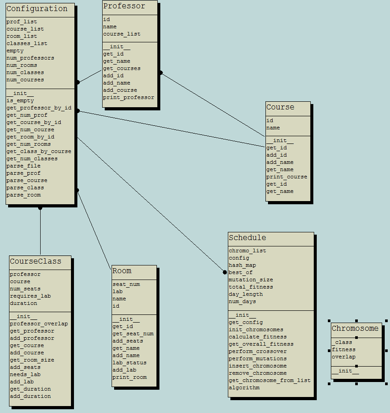
\includegraphics{classDiagram.png}
\caption{Class Diagram of Algorithm}
\end{figure}

% Perhaps there could be a diagram for the below.
The interaction diagrams below contain interactions of each user: student, lecturer, program manager, and program administrator. Each diagram details a pictorial representation of the user: interaction with the system, such as the website, the Django engine, the database that handled, or the algorithm itself.  In all these diagrams, the portal, or front-end website, is an input/output object wherein users will input items and receive output from Django. From behind the front-end website, Django serves as a control object that handles all aspects of user, algorithm, and database interactions. The database itself is an entity that stores information from user input processed by Django, and it also provides output to the user. Lastly, the algorithm is a control entity that manipulates the database courses, but all functionality of the algorithm remains hidden from the entire system. 
\pagebreak
\begin{figure}[!h]
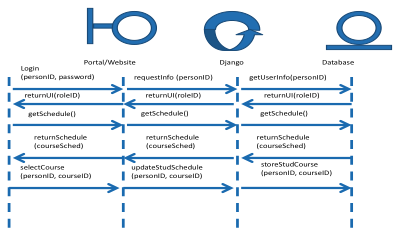
\includegraphics{studentID.png}
\caption{Student interaction diagram}
\end{figure}
\pagebreak
\begin{enumerate}
\item The student will login with their ID and password on the portal. Django will read the ID and password and match it with the database. 
\item Once the database confirms user, the database will return the correct UI for the student.
\item The student will want to get the schedule of classes to sign up for and makes a request to Django and the database to display the available courses. By making a request, this is done invisible to the user and the user will simply click on the courses tab. It will open automatically for the user. 
\item The student can now select courses and store them into their profile on the database. 
\end{enumerate}

\begin{figure}[!h]
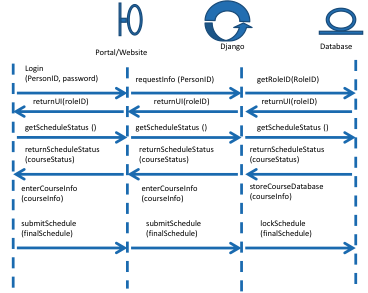
\includegraphics{programAdminID.png}
\caption{Program Admin enters courses interaction diagram}
\end{figure}

\begin{enumerate}
\item The program administrator will login with their ID and password on the portal. Django will read the ID and password and match it with the database. 
\item Once the database confirms user, the database will return the correct UI for the program administrator.
\item The program administrator will want to know the status of the schedule, to see if it is finished or not, and will make a request to both Django and the database to find out the status. 
\item The database will return the status. 
\item The program administrator will begin filling out course information through a courseInfo object that will contain various data about a given course.
\item When the program administrator feels done, they can choose to submit the course and lock the course in the database. 
\end{enumerate}

\begin{figure}[!h]
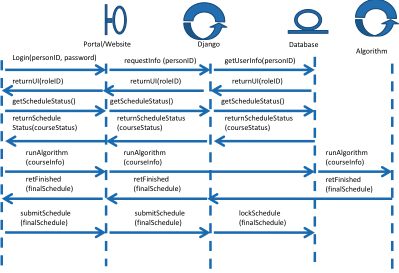
\includegraphics{programAdminID2.png}
\caption{Program Administrator runs algorithm interaction diagram}
\end{figure}

\begin{enumerate}
\item The program administrator will login with their ID and password on the portal. Django will read the ID and password and match it with the database. 
\item Once the database confirms user, the database will return the correct UI for the program administrator.
\item The program administrator will want to know the status of the schedule, to see if it is finished or not, and will make a request to both Django and the database to find out the status. 
\item The database will return the status to see if the program manager has completed the schedule. 
\item If the schedule is complete, the program administrator will run the algorithm that will be passed through Django and straight into the algorithm engine.
\item When the engine has completed, it will return a message that it is complete to the HTML website. 
\item Once the program administrator reviews the schedule, the program administrator can submit and lock the schedule and provide it to students
\end{enumerate}

\begin{figure}[!h]
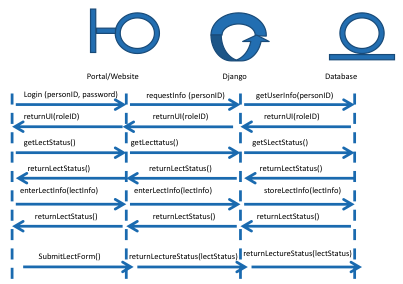
\includegraphics{lecturerID.png}
\caption{Lecturer interaction diagram}
\end{figure}

\begin{enumerate}
\item The lecturer will login with their ID and password on the portal. Django will read the ID and password, and match it with the database. 
\item Once the database confirms user, the database will return the correct UI for the lecturer.
\item The lecturer will want to find out the constraint form has been completed. Upon logging in, Django will send a message on the status of his constraint form, based upon a status in the database.
\item The lecturer will fill out the constraint form and store it in the database.
\item Upon storing it in the database, the lecture status will be updated and confirmed. 
\item The lecturer can now formally submit his constraints form to the database. 
\end{enumerate}

\begin{figure}[!h]
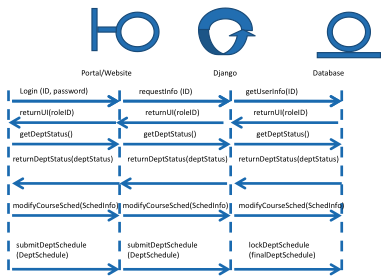
\includegraphics{programManagerID.png}
\caption{Program Manager interaction diagram}
\end{figure}

\begin{enumerate}
\item The program manager will login with their ID and password on the portal. Django will read the ID and password and match it with the database. 
\item Once the database confirms user, the database will return the correct UI for the program manager.
\item Upon logging in, Django will automatically send a request to find out the department status of the courses. 
\item If the status is not yet been completed, it will send a message to the program manager.
\item The program manager can modify the courses that was made available from the program administrator and placed in the database. 
\item Upon modifying the courses and the course info, the program manager can confirm and submit the finalized course. 
\end{enumerate}


\section{Architectural Design} % Erik
Our architecture is broken into three main categories:
\begin{enumerate}
\item User interface or UI (The front end)
\item Django (The back end)
\item The Scheduler (The engine)
\end{enumerate}

\subsection{The User Interface}
There are four different user interfaces, each is assigned to one of the four roles that a user could be: Program administrator, program manager, lecturer, student. The students UI is the most complex and offers the most customization.

The program administrator's user interface is fairly simple, they are given fields such as courses, rooms, and professors to fill out, once they fill out the fields to the proper specifications for the quarter then they have an option to run the scheduler. The scheduler will run, and then post the results to the program manager.

The program manager's interface will display all of the courses and lecturers for their department. The program manager will have the option of selecting the lecturers and courses that they want to be active for the quarter.

The lecturer will have an interface that will hold the courses that they can teach and the current courses that they are teaching. 
The student will have a customizable interface which will hold their past, present and future schedules. It will also have other widgets that they will be able to add to their profile.
\subsection{Django}
Django connects the user interface, the database and the scheduler. Django manages the user interface by handling the user requests and providing the appropriate response. In the case of the scheduler it takes the request from the program administrator to run the scheduler and creates a request object and sends it through multiple middlewares (Python functions). Django then checks the URLs and determines which function it must send the request object. The function in this case is the scheduler, which takes the information stored in the program administrators database and runs. The output of the scheduler is placed into a second database and the request object is sent back up through the middleware in the reverse order of the way it came in. The second database is then displayed to the program administrator.

\subsection{The Scheduler}
The algorithm we use is a modified genetic algorithm, which mimics the process of natural selection in order to find the solution to our scheduling problem. The algorithm represents the variables as chromosomes. A full set of chromosomes make up a parent, each parent is given a fitness value according to how well they fit into the schedule. Fitness is higher for matches that fit into empty classrooms, have the appropriate number of seats, or if the class has a lab in it. The parents make up a population, the algorithm takes 'n' number of parents from the population and does a crossover on pairs of the selected parents to create 'n' new chromosomes. The algorithm replaces 'n' chromosomes from the existing population with the new chromosomes that were created by the crossover, however it does not replace the chromosomes with the best fitness. After the crossover is performed, mutations take place. A random number is generated, which represents the mutation size. While the size has not been reached, classes are moved at random to a random room. Classes with the best fitness are ignored. The algorithm repeats this process until it reaches a fitness of one, in which has it has found an optimum solution. The algorithm pulls information from the database, and enters it into four different list: a professor list, a course list, a room list and a classes list. It then outputs into a second database which is then displayed to the user interface.

\section{Project Plan} % Justin

The project plan will describe the date and deliverables of our development process. The SCORE project followed a software methodology course and many of the deliverables are similar to those in the SCORE requirements. 

Instruction and classes began on September 23, 2010 and would continue for 10 weeks until the end of the quarter. Further development of our scheduling system will continue on to the winter quarter starting January 4, 2011 through March 18, 2011. 

\subsection*{Week 1: Initial Presentation}

For the first week, we had to gather in groups of 5 to form teams for our project and give an initial presentation on a brief overview of our project. 

We covered the following items:
\begin{itemize}
\item Team name
\item Team members
\item User experience
\item Core functionality
\item Wish list
\item Possible project risks
\end{itemize}

\subsection*{Week 2: Requirements - Scenarios}

During this week, our team designed several user scenarios related to our project. The scenarios will be a significant part of our requirement document and will be important in defining various aspects of our system�s functionality. We came up with 5 user scenarios:  (2) program administrators, program manager, lecturer professors, and students. 

Each scenario outlined and described the end user�s interaction with the system, the data flows of information, and the interaction with different functions and systems as the user performed a particular action. 

\subsection*{Week 3: Requirements - Complete}

After defining our scenarios, we created a complete and defined requirements document which will be necessary for implementing our system in a clear and concise matter. It details the specification of the functionality and constraints on that functionality for our scheduling system. 

The requirements we cover include the following:
\begin{itemize}
\item Functional - A specific and detailed description and list of what our system is
\item Performance - Specific characteristics of the performance of our system
\item Usability - How users interacts with our system
\item Wish list - System features we hope to implement if time permits
\item Coding Standards - Rules for organizing and formatting code
\item Preliminary User interface - Preliminary sketch drawings of what our user interface will look like. 
\end{itemize}
In this week, we also had to give a Design Presentation which will basically outline everything in our requirement documents and how it is done. 

\subsection*{Week 4: Architecture and Design Document}

After defining our requirements and scenarios, we create an architecture and design document that will document the high-level architecture and the detailed design of our project. It will have a detailed description of the objects that we will use as well as relationships between objects. 

We created the following items: 
\begin{itemize}
\item Overview - The overview document will provide context and an overview of our diagrams. It will include description of our major design decisions and modularization criteria. 
\item Architecture diagram - High-level overview of the components in our system and how they co-operate. 
\item UML Structure diagrams - Diagrams of our class objects in the form a UML structure diagrams that describe the attributes and operations.
\item UML Interaction Diagrams - A developed UML diagram based on several of our scenarios we produced for our requirement documents. 
\end{itemize}
\subsection*{Week 5-6: Development and user manual}
During this phase of our course, implementation of our system was to commence and continue for the next several weeks. This includes implementing our design and requirement documents. As we were creating this system, we were also simultaneously required to create a user manual that details how our system is to work. The user manual was broken down into the following parts:
\begin{itemize}
\item Purpose - Description of the UI and functionality 
\item How do you do this? - Defining user classes, convey the user experience level at each of the classes,  and provide computerized help.
\end{itemize}

\subsection*{Week 7: Software inspection}

A software inspection is an in-class �presentation� where our group simultaneously and systematically reads source code and identifies and classifies defects as they are encountered. For our software inspection, we chose our algorithm class that will be the primary engine that will run our course scheduling system. 

It is also important to note that a software inspection is strictly a time to catch defects and not make an attempt to discuss how to fix it or what to do to fix it. There is no discussion of the problem at this time, it is simply to define the problem and make note of it to the developer. 

\subsection*{Week 8: Unit Test}

Our group created several unit tests that tested the various classes and modules of our system. These consisted of simple script code that automated and simplified testing for us. Since our project was primarily written in the context of Django's framwork, we created very simple Python scripts that quickly tested each software component and its expected responses. 

\subsection*{Week 9-10: Acceptance Test}

With our development, testing, and inspection complete, we demonstrate our system to our primary stake-holder (our professor). An acceptance test is generally a basic run-through of our entire end-to-end user experience of our system. 
At this point, the quarter is about to end and all our project deliverables should have been completed and ready to be delivered as a final product. Due to the scale of our particular project, we unfortunately did not have a complete end-to-end system. However, bits and pieces of our system worked well when isolated. 

Because our system was incomplete at this point, we decided to spend the next academic quarter completing development of our project. The next academic quarter at UC Santa Cruz would not begin until January 4, 2011 and would end on March 18, 2011. The following is our tentative plan for the second quarter. 

\subsection*{Week 1: Review}

Our plan is to review our system and deliverables. We define items we need to complete or improve on. We also make the decision to revise our life cycle model from Unified Process to an agile Scrum software methodology. We plan on holding short meetings every evening to update each other with any new progress, along with weekly planning meetings where we sit down and discuss future development. 

\subsection*{Week 2: Documentation improvement}

With our SCORE submission coming near, we focus this week on writing the report. After this week has concluded, we'll continue development on our project.

\section{Management Plan} % Erik and Will
Because the skill sets of our team members were remarkably heterogenous, proper management of our team was crucially important as it allowed us to delegate work that we considered specialized to the proper specialist on our team in order to complete work in an efficient manner.

\subsection{An Overview of the Management Process}
Our teams' management has been primarily democratic; the management is broken into two timeframes corresponding to our schools quarter system. For the first part of our project we would meet for class twice a week and at least once outside of class. Meetings kept our team on the same page and allowed us to coordinate our project efforts.

It took weeks for us to each fall into our individual roles. For the first couple of phases of the project we were all involved in deciding how we were going to structure our system and what needed to be done. We would meet in class and discuss the best options from the research everyone had done before class and then work in pairs or individually until our next class meeting. It wasn't until the implementation phase that we each chose specific parts of the project that we would each work on. 

We finished our first acceptance test before winter break; over the break we all had a chance to look at the code that our team mates had written so that we would all be familiar with all aspects of the project.
 
After the break our management plan was revised. We switched over to the Scrum process, and we now are meeting once a day for fifteen minutes. Additionally, Will took over as project manager, and has taken on the responsibility of coordinating our meetings and resolving any issues that prevent team members from making progress. 
	
\begin{description}
\item{\textbf{Ben Ross}} - In charge of coding the algorithm
\item{\textbf{Professor Charlie McDowell}} - Project reviewer
\item{\textbf{Erik Steggall}} - In charge of connecting Django and the scheduler
\item{\textbf{Justin Lazaro}} - In charge of documentation
\item{\textbf{Professor Linda Werner}} - Project reviewer
\item{\textbf{Sabba Petri}} - In charge of the user interface
\item{\textbf{Will Crawford}} - In charge of Django administration and overall expertise
\end{description}

\subsection{Channels of Communication}

\begin{description}
\item{\textbf{Subversion (SVN)}} \\As part of the class, we were required to use Subversion as a project repository for our code, as well as other deliverables for the class. Subversion is a source control mechanism that allows multiple people to remotely collaborate on the same codebase. We used Subversion to transfer code and miscellaneous files between team members. We also used it to automatically merge source code files.
\item{\textbf{Google Groups}} \\For the purposes of communicating by e-mail, we created an e-mail list with Google Groups; it allowed us to automatically archive our e-mail conversations and bounce all communication to each team member. Scheduling meetings was done primarily via this e-mail list. It also initially served as a rudimentary feature tracker.
\item{\textbf{Daily Skype Meetings}} \\After the conclusion of the class, we continued to meet via Skype every night for 15 minutes to check in with each other. These meetings were intended to briefly answer three questions: ``What did you work on today?'' ``What are you working on tomorrow?'' and ``Is there anything preventing you from making progress?''
\item{\textbf{Git \& Codaset}} \\After the class concluded, we switched from Subversion to Git as more of our team members were comfortable with it and preferred it. Git is another source control mechanism, but we found its granularity regarding which files it committed to be superior to that of Subversion. We also found its merging algorithm produced fewer conflicts during our usage. The website Codaset \texttt{(http://codaset.com/)} served as a central repository for the highly mobile team, as well as a GUI for viewing the repository's metadata, such as commit histories, volume, etc.
\end{description}

\section{Implementation} % Ben

Implementation of the MyCourses scheduling system was a multifaceted problem. The overall system was broken down into four main parts to implement: Web Interface, Database, Algorithm, and Security. Our implementation strategy was to find the best way to implement the parts separately, and then collectively integrate them together. This would allow us to selectively work on each part of the combined system separately.

The front end of our system was written in HTML and CSS. We decided to use Javascript to add functionality to the front end because it is widely supported and renders much faster than Flash. In addition, unlike Flash, Javascript is rendered in browsers without a plugin.

The Django framework was selected for a few reasons. Django has an interface that allows for robust database operations without , as well as Pythonic template systems to display information on varying web pages. This allows us to integrate the algorithm with the database seamlessly. This was to be a major problem facing our system, but was quickly alleviated earlier in the process. Django uses forms and templates to display information from the database to web pages and this allows us to create a few templates for each of the authentication levels, all of which are able to display information directly from the database with no SQL queries. Because Django performs operations on the database transparently, Python queries are performed with great speed, letting pages load quicker. % Is this last sentence true?

The Algorithm went through three different implementations before the best implementation was selected. The first implementation was a slow Algorithm designed by one of the team members. It was very inefficient, but allowed the program administrator complete history of the courses that were scheduled at a given time, in a given room. This allowed for easier manual edits of the proposed schedule. The second implementation was using a FLOSS constraint-solver Minion. This solution was very fast, but needed a complicated script to translate from the database to the solver and back again. The third implementation was a scheduling algorithm using a genetic Algorithm. This Algorithm was based off of a freeware genetic algorithm scheduler. The Algorithm was written in Python, allowing it to be fast and easily modifiable. The genetic Algorithm was selected as the best implementation solution, because it allowed seamless integration with the database, and it proves incredibly fast, even for larger solutions.

Security for our system was not something that came up in our initial discussions of the system. However, security is one of the most important aspects of a web application. Also, universities generally have lots of sensitive data displayed on similar applications and thus, security needs to be paramount. The security system we designed into our system also integrates with the privacy settings for the application. HTTPS is used instead of the HTTP; this allows all traffic coming to and from the system to be encrypted. This is a step above popular web applications like Facebook, and Myspace, providing students, faculty members, and administrators peace of mind, knowing their traffic will be very difficult to decrypt. Our second important security feature is passwords. Our minimum password length is 8, with a minimum of one capital letter, one symbol, and one letter. This allows users increased security from brute force password attacks. Another security feature involving passwords is similar to what some banks do. We assign each user a sitekey, which is a random picture out of 50. The user is then requested to name the sitekey. When the user enters their password, if an incorrect sitekey is displayed, the user is made aware of an attempt to compromise their information. 

The other security features deal with the privacy of the user once they are in the system. These features are designed for the student role only. The integration of Facebook with our system provided another way for our system to lose security. When the student first logs into the system, a tutorial walks them through setting up their account and linking it with their Facebook. The student has the option to turn off sharing of information during this setup, as well as, anytime through the account settings page. This feature gives permission to students for complete access as to what information they share through our system, and through Facebook. Allowing students this control will decrease the chances of a student sharing more information than they previously wanted to.

\section{Validation and Verification} % Ben and Erik
Our test framework for our implementation has three forms. Testing for the algorithm, testing for the web UI and testing the database through Django. The testing for the algorithm is done by scripts, and the web UI testing is done through a software suite and testing Django is done through Django's testing suite.

The algorithm was first tested by running the algorithm and then manually checking the output. The output was checked to see if the proposed schedule was a valid schedule and to see if all of the constraints were met. This became very tedious for large class schedules, so a script was written that validates the output based on the constraints given in the database. This allowed large testing to be completed much faster.

The web UI testing is done using a framework called Selenium. This open source tool allows automatic testing of the web UI. Two methods were used for writing tests for the web UI. Selenium has an IDE that allows you to record an interaction with the web UI and
run that recording as a test. This was done for basic actions, such as logging in and out. The other way our python scripts that use Seleniums built in libraries to interact with the web interface. This allows the tester to check for output on a given page and to
perform more complex actions. This was done for advanced actions, such as signing up for classes, or adding students to the database.

Django's testing is done through tests.py. Django's test suite can test the framework with and other utilities. The testing suite is split into two different sections; doctests and unit tests. The tests are run through pythons manager, it can test the entire framework, or specific modules of it. Our project used the unit test portion of the test suite to test the database and the database to algorithm connection.

\section{Outcomes and Lessons Learned} % All
\subsection{Ben Ross}
Throughout the development of the MyCourses system, I learned a few valuable lessons. The first being that there is no one correct development process for a given system. For 10 weeks we developed out system using the Unified Process, only to shift over to the Agile process called Scrum. This shift highlighted all of the problems that we were having with the Unified Process, and alleviated most of them. The second lesson I learned is to try to select technology that team members have familiarity with. Throughout the development process our team has used countless tools and programs to aid in our development and management. No one tool, like development processes, is able to provide a complete solution to our problems. This brings up the question of whether or not we are the only team to encounter such a problem, and if this problem could be solved; however, that is not the focus of this paper. Our current iteration of software tools seems to be the best iteration yet. This judgement is based on 4 previous iterations, and takes into account the development process switch. Overall what I have learned from the development of this project will greatly aid my fellow teammates and myself in our future classes and careers.

\subsection{Erik Steggall}
The most valuable part of working on this project was learning how to work as a team for a software project. Before I started this project I had no idea how a software development team would work, programming was mostly a solitary experience. Over the course of this project I have learned about how to manage and function in a working development team. I find that working on a software project is difficult to manage; members have their own different schedule and skill set that needs to be held into consideration. In order to not get out-of-sync with each other there need to be proper lines of communication. Our current method of meeting everyday is working better because it keeps everyone up to date with the project. However, we keep the meetings short so that they are not too overwhelming. This project has taught me how to work in a functioning development team which will be invaluable in the future.

\subsection{Justin Lazaro}
One of the most valuable lessons from this project is that tailoring a specific life-cycle model is in fact a very important aspect in software engineering and it is a aspect that I have not previously taken into account when developing software. For the first several weeks of development we initially utilized the waterfall lifecycle model. It quickly proved to not be the ideal way of developing software for our particular project and purposes. Because a lot of what we were implementing was relatively new to us, we felt the agile method was more appropriate and better suited for us. I also came to really appreciate utilizing models to graphically represent how we intend to build our software.
% We never used the waterfall method. =|

\subsection{Sabba Petri}
One of the lessons learned later in the development process was our failure to understand each other�s individual strengths from the beginning. Having known each other�s individual strengths from the outset, we could have played to our strengths and allocated the jobs in a more effective manner. For example, teammate A has a strong background in web programming, as well as Python, while teammate B solely has a strong background in Python. Because of our lack of foresight in this department, teammate A took majority of the Python programming, while teammate B was left to aid him, as well as work on other aspects of the project, including web programming. What should have happened was, teammate B should have worked on the Python aspect of it, while teammate A could have aided him, as well as worked on other parts, such as web programming or even with other parts of the back-end.  This would give more help, as teammate A has more use in multiple areas rather than one general area. Though we did recount in the beginning our strengths, they could have been played out better, and this was something we learned a bit deeper in the process.

\subsection{Will Crawford}
I learned a lot about project collaboration. For the entirety of this project, there have been technologies that we've been using that at least one of our member's didn't understand. One lesson I took from this is that a hands-on demonstration can often teach someone to use a technology much faster than providing documentation can, even if that documentation is very complete. Another lesson was that distributing that understanding across the entire team is not always necessary. Rather than having everyone put equal work into all parts of the project, it often makes more sense to leave one facet of the project to someone who knows what they're doing and have other team members work on the parts that they are, in turn, good at doing.

I also learned that new technologies can be somewhat inscrutable. Toward the beginning of the project, it was very difficult to grasp what would be easy to do with the technologies we were going to use, and what would be difficult. Having a good grasp of the technologies we were going to use would have greatly accelerated our elaboration phase.

\end{document}
